


\tikzset{every picture/.style={line width=0.75pt}} %set default line width to 0.75pt        

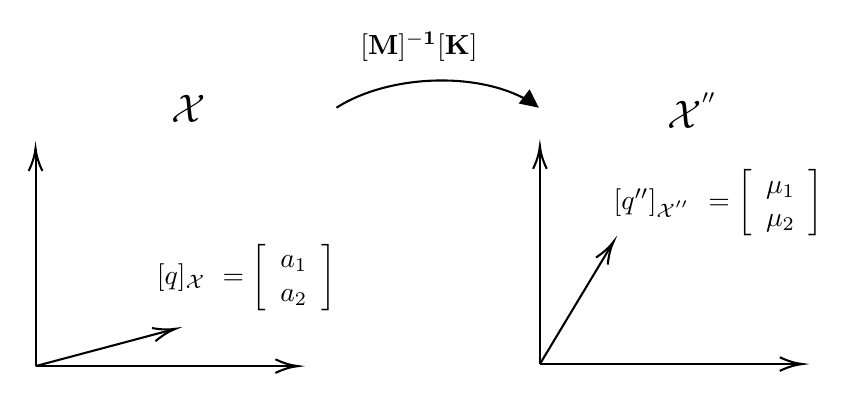
\begin{tikzpicture}[x=0.75pt,y=0.75pt,yscale=-1,xscale=1]
%uncomment if require: \path (0,15225); %set diagram left start at 0, and has height of 15225

%Straight Lines [id:da46971419391016966] 
\draw    (155,5164) -- (155,5061) ;
\draw [shift={(155,5059)}, rotate = 90] [color={rgb, 255:red, 0; green, 0; blue, 0 }  ][line width=0.75]    (10.93,-3.29) .. controls (6.95,-1.4) and (3.31,-0.3) .. (0,0) .. controls (3.31,0.3) and (6.95,1.4) .. (10.93,3.29)   ;
%Straight Lines [id:da03406383173301375] 
\draw    (155,5164) -- (279.5,5164) ;
\draw [shift={(281.5,5164)}, rotate = 180] [color={rgb, 255:red, 0; green, 0; blue, 0 }  ][line width=0.75]    (10.93,-3.29) .. controls (6.95,-1.4) and (3.31,-0.3) .. (0,0) .. controls (3.31,0.3) and (6.95,1.4) .. (10.93,3.29)   ;
%Straight Lines [id:da6733447176724459] 
\draw    (398,5163) -- (398,5060) ;
\draw [shift={(398,5058)}, rotate = 90] [color={rgb, 255:red, 0; green, 0; blue, 0 }  ][line width=0.75]    (10.93,-3.29) .. controls (6.95,-1.4) and (3.31,-0.3) .. (0,0) .. controls (3.31,0.3) and (6.95,1.4) .. (10.93,3.29)   ;
%Straight Lines [id:da7503857823126457] 
\draw    (398,5163) -- (522.5,5163) ;
\draw [shift={(524.5,5163)}, rotate = 180] [color={rgb, 255:red, 0; green, 0; blue, 0 }  ][line width=0.75]    (10.93,-3.29) .. controls (6.95,-1.4) and (3.31,-0.3) .. (0,0) .. controls (3.31,0.3) and (6.95,1.4) .. (10.93,3.29)   ;
%Straight Lines [id:da495111073609535] 
\draw    (155,5164) -- (220.57,5146.52) ;
\draw [shift={(222.5,5146)}, rotate = 165.07] [color={rgb, 255:red, 0; green, 0; blue, 0 }  ][line width=0.75]    (10.93,-3.29) .. controls (6.95,-1.4) and (3.31,-0.3) .. (0,0) .. controls (3.31,0.3) and (6.95,1.4) .. (10.93,3.29)   ;
%Straight Lines [id:da7833684320650613] 
\draw    (398,5163) -- (432.47,5105.71) ;
\draw [shift={(433.5,5104)}, rotate = 121.04] [color={rgb, 255:red, 0; green, 0; blue, 0 }  ][line width=0.75]    (10.93,-3.29) .. controls (6.95,-1.4) and (3.31,-0.3) .. (0,0) .. controls (3.31,0.3) and (6.95,1.4) .. (10.93,3.29)   ;
%Curve Lines [id:da4396149957962707] 
\draw    (300,5039.5) .. controls (325.71,5023.01) and (371.17,5021.57) .. (395.32,5037.93) ;
\draw [shift={(397.5,5039.5)}, rotate = 217.45] [fill={rgb, 255:red, 0; green, 0; blue, 0 }  ][line width=0.08]  [draw opacity=0] (8.93,-4.29) -- (0,0) -- (8.93,4.29) -- cycle    ;

% Text Node
\draw (458,5031) node [anchor=north west][inner sep=0.75pt]  [font=\Large]  {$\mathcal{X}^{''}$};
% Text Node
\draw (219,5032) node [anchor=north west][inner sep=0.75pt]  [font=\Large]  {$\mathcal{X}$};
% Text Node
\draw (212,5104) node [anchor=north west][inner sep=0.75pt]    {$[ q]_{\mathcal{X}} \ =
\left[
\begin{array}{c}
a _{1}\\
a _{2}
\end{array} 
\right]  $};
% Text Node
\draw (432,5068) node [anchor=north west][inner sep=0.75pt]    {$[ q'']_{\mathcal{X}^{''}} \ =
\left[
\begin{array}{c}
\mu _{1}\\
\mu _{2}
\end{array} 
\right] $};
% Text Node
\draw (310,5001.5) node [anchor=north west][inner sep=0.75pt]    {$\mathbf{[M]^{-1}}\mathbf{[K]}$};


\end{tikzpicture}
